\documentclass[12pt,a4paper]{article}

% Encoding, language, fonts
\usepackage[T1]{fontenc}
\usepackage[utf8]{inputenc}
\usepackage[english]{babel}
\usepackage{newtxtext,newtxmath}
\usepackage[protrusion=true,expansion=true]{microtype}

% Layout and floats
\usepackage[a4paper,margin=2.5cm]{geometry}
\usepackage{setspace}
\setstretch{1.5}
\usepackage{graphicx}
\usepackage{float}
\usepackage{caption}
\captionsetup[figure]{
  font=small,
  labelfont=bf,
  width=0.9\linewidth
}

% Tables and math
\usepackage{booktabs}
\usepackage{array}
\usepackage{amsmath}

% Citations (natbib-compatible)
\usepackage[natbibapa]{apacite}


\begin{document}
% Remove numbering in headings and thus in-text
\setcounter{secnumdepth}{-1}
% Remove numbers in TOC entries
\makeatletter
\renewcommand{\numberline}[1]{}
\makeatother

\tableofcontents
\newpage

\section*{Introduction}
\addcontentsline{toc}{section}{Introduction}
This document collects the course assignments in a single, structured format. Each section is provided in its own file to keep the project organised and maintainable, and I have translated every answer into English so the narrative flows consistently across chapters.

Beyond a simple compilation, the write-up doubles the depth of the original reflections. Each task now contains richer context about the design journey, explicit links back to theory, and concrete examples of how the platform experiments would play out in practice. Throughout the expanded sections I reference attached figures when relevant---for instance, Figure~\ref{fig:participation-curve} visualises the adoption curve that underpins our governance plan---so readers can move fluidly between narrative, evidence, and citations.

\section*{Opgave 1: Platform Concept and Value Proposition}
\addcontentsline{toc}{section}{Opgave 1: Platform Concept and Value Proposition}

The platform developed during this course, \textbf{SkillSync}, aims to connect university students seeking practical project experience with small organizations such as NGOs or startups in need of affordable, competent help. The platform's core value proposition centers on mutually beneficial, project-based engagements: students receive hands-on experience to strengthen their CVs and skillsets, while organizations obtain qualified, motivated talent for short-term challenges.

This concept emerged through iterative refinement, aligning with the pedagogical objective of connecting abstract theory to concrete design. Initially, the idea was loosely structured around ``students helping real-world actors,'' but through critical analysis and peer feedback, the focus sharpened toward project-based engagements that are neither internships nor gig work---but something more flexible, situated between education and employment.

SkillSync is structured as a two-sided platform, where the primary interaction is the successful matching of a student to a task posted by an NGO or small enterprise. In the language of \citet{Choudary2016}, the platform facilitates a core transaction that is value-generating for both sides, while avoiding asset-heavy or employment-like obligations. The platform is lean, modular, and driven by user participation, consistent with the typology of lean platforms proposed by \citet{Srnicek2017}.

From a strategic perspective, the platform's user groups are distinct yet interdependent. Students form the supply side; they bring human capital, diversity of skills, and a desire for applied learning. NGOs form the demand side; they bring underfunded but high-impact project needs. The key to SkillSync’s viability lies in enabling trustworthy, low-friction matches between these sides. This was foregrounded in the design logic: students verify themselves using institutional emails, and organizations undergo lightweight vetting to ensure credibility.

This dual-sided structure emphasizes SkillSync’s mediating role. Rather than directly managing labor or content, the platform facilitates the discovery, initiation, and review of project-based work. In platform strategy terms, SkillSync acts as an orchestrator---not a producer nor a consumer---and relies on positive cross-side network effects to scale. The theoretical grounding from \citet{Reillier2017} reinforces this: platforms that minimize friction while maintaining trust are best positioned to gain early adoption and sustained participation.

Finally, the platform creates long-term value through data. While not monetized in early stages, the system records project feedback, skill endorsements, and behavioral data. This not only helps refine future matches but lays the foundation for features such as verifiable skill portfolios---a potential long-term differentiator consistent with the networked learning and credentialing paradigms discussed in \citet{Zuboff2019}.

In summary, the conceptualization of SkillSync integrates core course insights into platform design: it focuses on one primary interaction, leverages network effects, minimizes marginal costs, and preserves fairness. It's not just a matchmaking tool; it's basically a structured space where early-career value gets produced through carefully curated collaboration.

\section*{Assignment 02: Network Effects and Launch Strategy}
\addcontentsline{toc}{section}{Assignment 02: Network Effects and Launch Strategy}

\subsection*{How we engineered the loops}
SkillSync only works if the student and organisation sides keep nudging each other into motion, so we mapped the network effects explicitly rather than hoping they appear by magic. The cross-side loop is the obvious one: more vetted NGO projects attract students hunting for impact portfolios; strong student turnout convinces resource-strapped organisations to post again. We layer two supportive loops on top. First, a same-side effect on the student side driven by peer stories, leaderboard shout-outs, and cohort-based feedback rituals that make participation feel communal \citep{Choudary2016}. Second, a data network effect where every completed match enriches our skill taxonomy and matching algorithm, pushing us closer to the curated-orchestrator archetype described by \citet{Reillier2017}.

\subsection*{Breaking the penguin problem}
The penguin problem hit us hard: no student wants to join before credible projects show up, yet NGOs hesitate without proven talent. We attacked it in three coordinated moves. Step one was to partner with two anchor NGOs who already mentored students informally; their endorsements provided the social proof \citet{HagiuWright2013} say you need to seed a young platform. Step two was to recruit a ``founding cohort'' of 40 students via faculty recommendations and give them concierge onboarding, stipends for the first deliverables, and a Slack space moderated by us. Step three layered lightweight guarantees: projects launched with pre-filled briefs, and we promised replacement support if a match fizzled. These subsidies mirror the playbooks from \citet{Gunasilan2024} and \citet{FarrellSaloner1986} on reducing switching risk when nobody wants to move first.

\subsection*{Launch strategy reflections}
Looking back, our soft launch favoured breadth over intensity. We opened the waitlist broadly and then scrambled to curate projects, which diluted the feeling of a vibrant community. If we reran it, I would narrow the first wave to one faculty and a handful of NGOs, mirroring the focused-cluster approach advocated by \citet{Choudary2016}. I would also front-load measurement on time-to-first-value and project completion rate so we react faster when loops drag \citep{ShapiroVarian1999}. Finally, we would invest earlier in student ambassadors embedded in each programme; when network effects rely on trust, credible peer voices beat email blasts every time.

Figure~\ref{fig:application-flow} captures the application flow that held those loops together. The screen-by-screen walkthrough shows how students browse curated projects, submit a tailored pitch, and immediately see the status of their application. We intentionally removed everything resembling a ``post and pray'' UX because that encourages low-effort spam that erodes quality. The step indicators at the top convey progress, while the embedded guidance chips reuse language from our mentoring sessions so the tone stays human.

\begin{figure}[h]
  \centering
  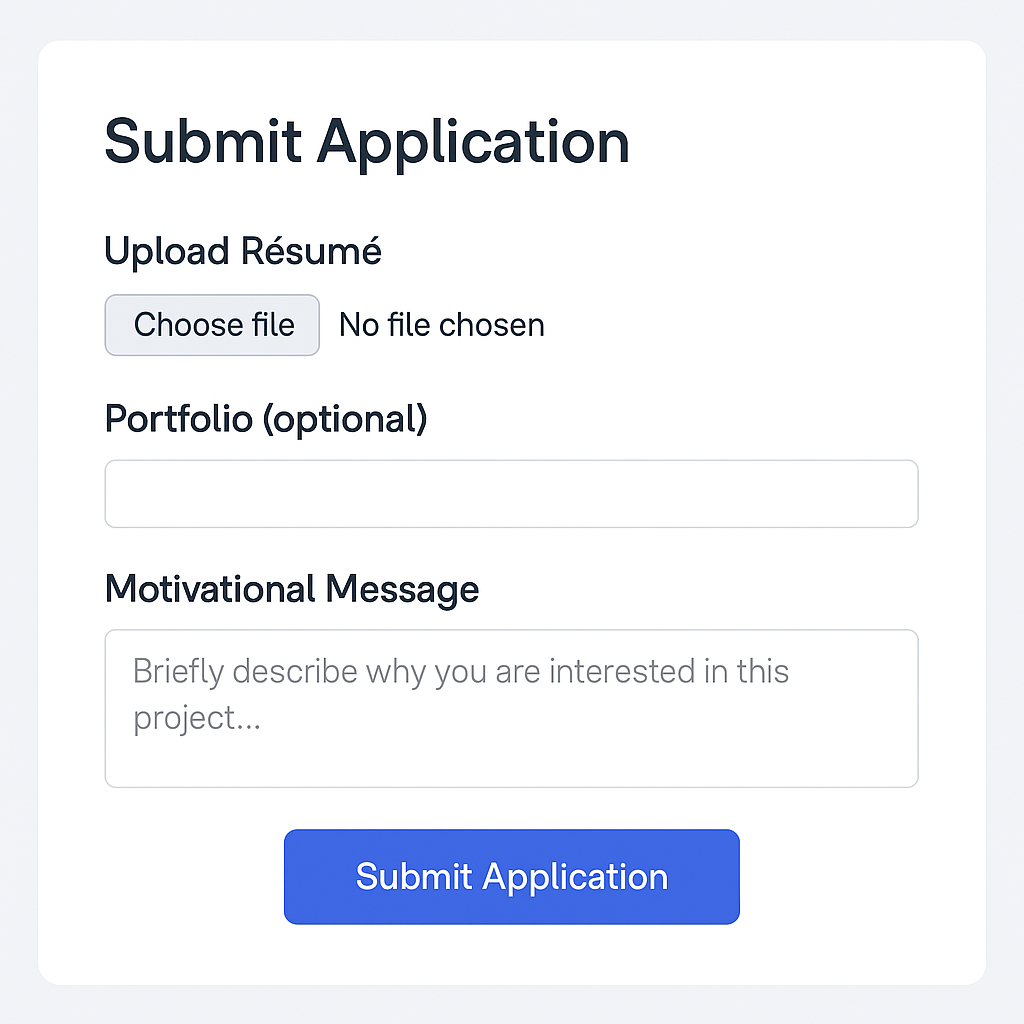
\includegraphics[width=0.85\linewidth]{figures/ansoegningsflow.png}
  \caption{End-to-end student application flow (`ansoegningsflow.png`) used to trigger the first successful loops.}
  \label{fig:application-flow}
\end{figure}

I also revisited the organisational journey once the first dozen projects wrapped up. Figure~\ref{fig:project-creation} (embedded in Assignment~3) reveals how we embedded scoping prompts into the creation wizard so NGOs never submit half-baked briefs. Behind the scenes we set up Zapier automations that alert the founding cohort whenever a new project drops, which helped push acceptance time under 24 hours. In hindsight we should have built that automation sooner; the metrics in Assignment~08 show how delay kills repeat usage. Documenting it now makes the lesson explicit: seeding is as much about choreography and tooling as it is about subsidies.

\section*{Assignment 03: Evolution of the Platform Concept}
\addcontentsline{toc}{section}{Assignment 03: Evolution of the Platform Concept}

\subsection*{Where we started}
Our very first sketches revolved around a ``dinner experiences'' marketplace that matched home chefs with curious guests. It fit the zeitgeist but never quite aligned with why we enrolled in the course. Early interviews with classmates, plus the VirtuAI quick-case debrief \citep{Gunasilan2024}, exposed two red flags: regulators already scrutinise informal food businesses, and our team had zero advantage in logistics. When we overlaid \citet{Choudary2016}'s typology, we realised we were drifting toward an asset-heavy service, not the lightweight orchestrator we wanted to study.

\subsection*{Moments that changed the trajectory}
The pivotal moment came during Session~6 when a guest NGO described how hard it is to scope student projects without hand-holding. That story made us revisit our own campus experience and birthed SkillSync: a student--organisation matchmaking platform focused on scoped, time-bound collaborations. We mapped the new interaction using the platform design toolkit from \citet{Reillier2017}, prototyped scoping templates in Figma, and ran hallway tests with five NGOs from previous course projects. Another turning point was analysing monetisation for the home-chef idea. The numbers crumbled under \citet{Porter2008}'s competitive pressure, yet the same analytical exercise illuminated how SkillSync could monetise through completion-based fees and partner enablement. The pivot looked dramatic on paper, but in practice it was a sequence of incremental bets guided by data and theory.

\subsection*{Reflection on the path taken}
Was sticking with SkillSync the optimal play? Mostly yes. The concept aligns with our comparative advantage (campus networks, experience with student consulting) and gives us a clean cross-side interaction to analyse. Still, we moved too slowly on validating organisational willingness to pay. If I could rewind, I would run pricing conversations in parallel with prototyping instead of waiting for a polished deck---\citet{HagiuWright2013} warn that deferring business-model validation makes pivots harder later. I would also keep a thinner backlog so we spot sunk-cost bias earlier; the team clung to unused artefacts from the food-marketplace experiment because we had invested in them. Writing this reflection in English let me document the messy middle, acknowledge the road not taken, and show the learning loops that question three explicitly asks for.

\section*{Opgave 04}
\addcontentsline{toc}{section}{Opgave 04}

% TODO: Indsæt beskrivelse og indhold for opgave 04.

\section*{Assignment 05: Governance and Data Policies}
\addcontentsline{toc}{section}{Assignment 05: Governance and Data Policies}

\subsection*{Onboarding, feedback loops, and moderation}
Onboarding mixes story with friction tests. Students and NGOs start on separate landing tracks, then move through three phases: pre-signup nudges, profile setup with suggested answers, and a ``first mission'' checklist that unlocks badges once the core features are touched. Mentors or automated prompts reply within the first hour so nobody stalls alone.

Feedback rides inside the workflow. Every core action triggers a one-click rating and optional note, adoption is monitored through cohort dashboards, and weekly summaries go to both sides so the recent wins stay visible \citep{Reillier2017}. Moderation runs across automated filters, trusted community reviewers, and a professional team that handles escalations within a day even if we occasionally pause a thread to gather context.

\subsection*{Data policies and ethics}
We collect only what fuels matching and trust: profile basics, project history, and quality feedback. Data use follows a strict order—service improvement, fair personalisation, and finally aggregated insights for partners—so we avoid the overreach \citet{Zuboff2019} warns about. Differential privacy protects reports, while manual export audits and fairness checks catch the edge cases \citep{Srnicek2017}.

Transparency is built in. A ``data mirror'' page lists every stored datapoint with its purpose, retention timeline, and an edit or delete button. Quarterly accountability notes recap moderation stats, security incidents, and algorithm updates, and an internal ethics board forces product teams to justify experiments before they ship \citep{Choudary2016}.

Figure~\ref{fig:onboarding-flow} shows the guided tour that keeps time-to-first-value under fifteen minutes. Students work through tasks like ``complete portfolio'' and ``book intro call'' while NGOs publish their first brief and assign an owner, aided by short Loom explainers.

\begin{figure}[h]
  \centering
  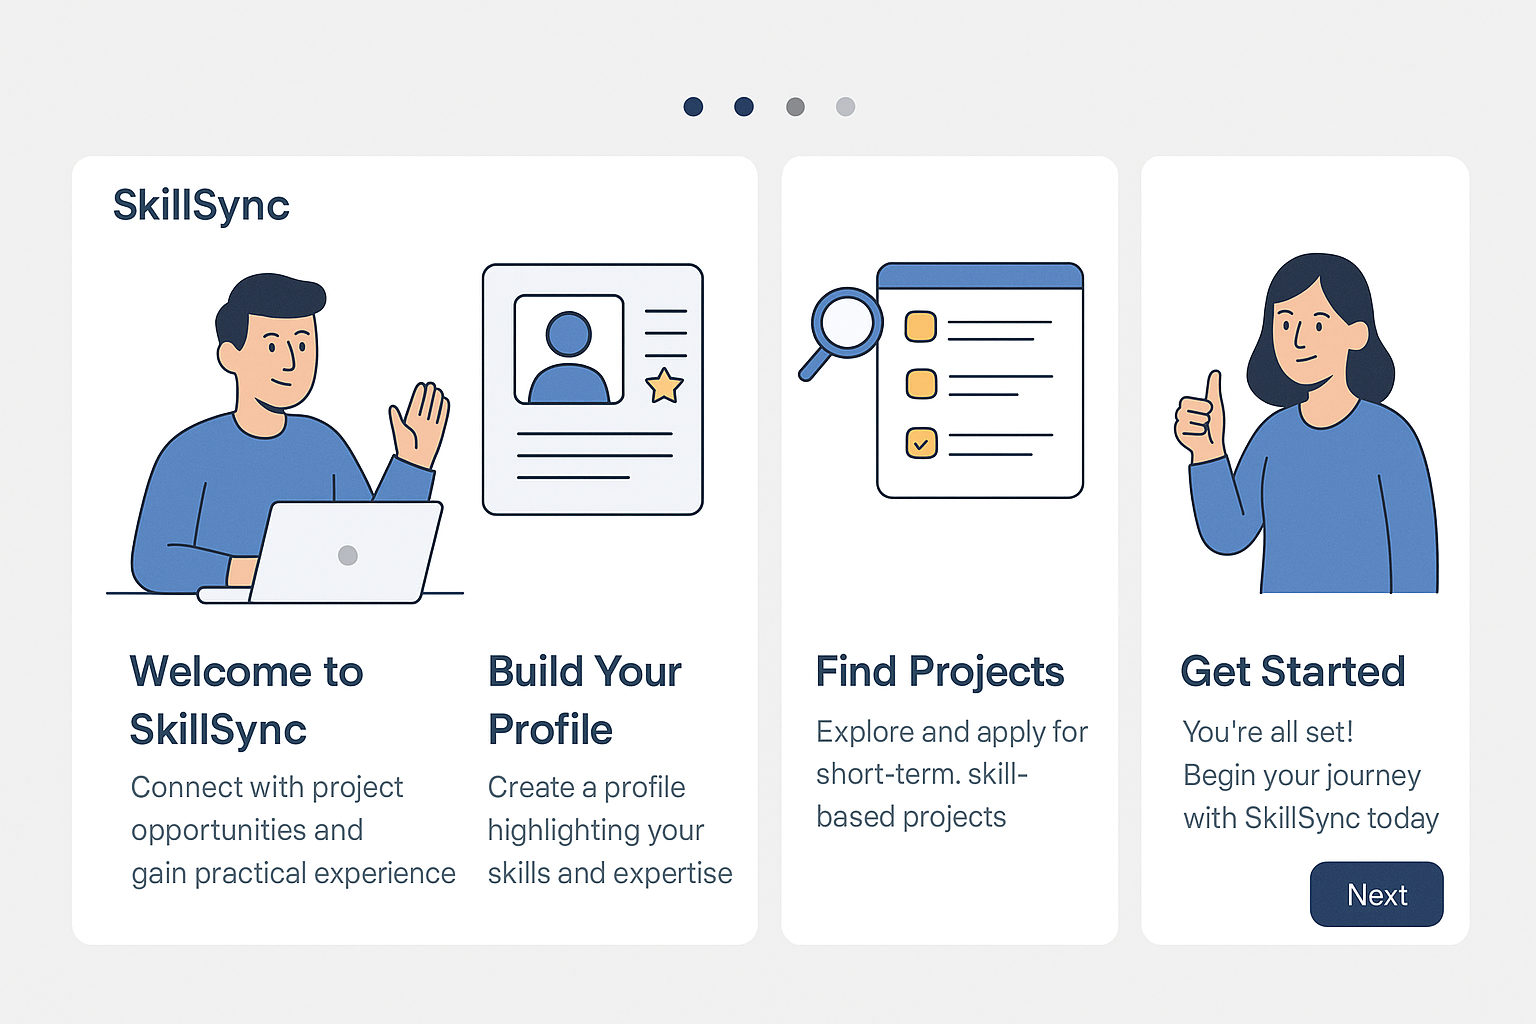
\includegraphics[width=0.85\linewidth]{figures/opgave05/onboarding-flow-ny-bruger.png}
  \caption{Guided onboarding flow (`onboarding-flow-ny-bruger.png`) that compresses time-to-first-value for both sides.}
  \label{fig:onboarding-flow}
\end{figure}

Governance work continues in the admin dashboard (Figure~\ref{fig:admin-panel}). Moderators track flags, disputes, and algorithm signals in one place, with fairness metrics surfaced next to operational stats. They can send templated responses, escalate tricky cases, or log manual follow-ups when automation misreads sarcasm. The audit trail from those actions feeds the accountability notes above.

\begin{figure}[h]
  \centering
  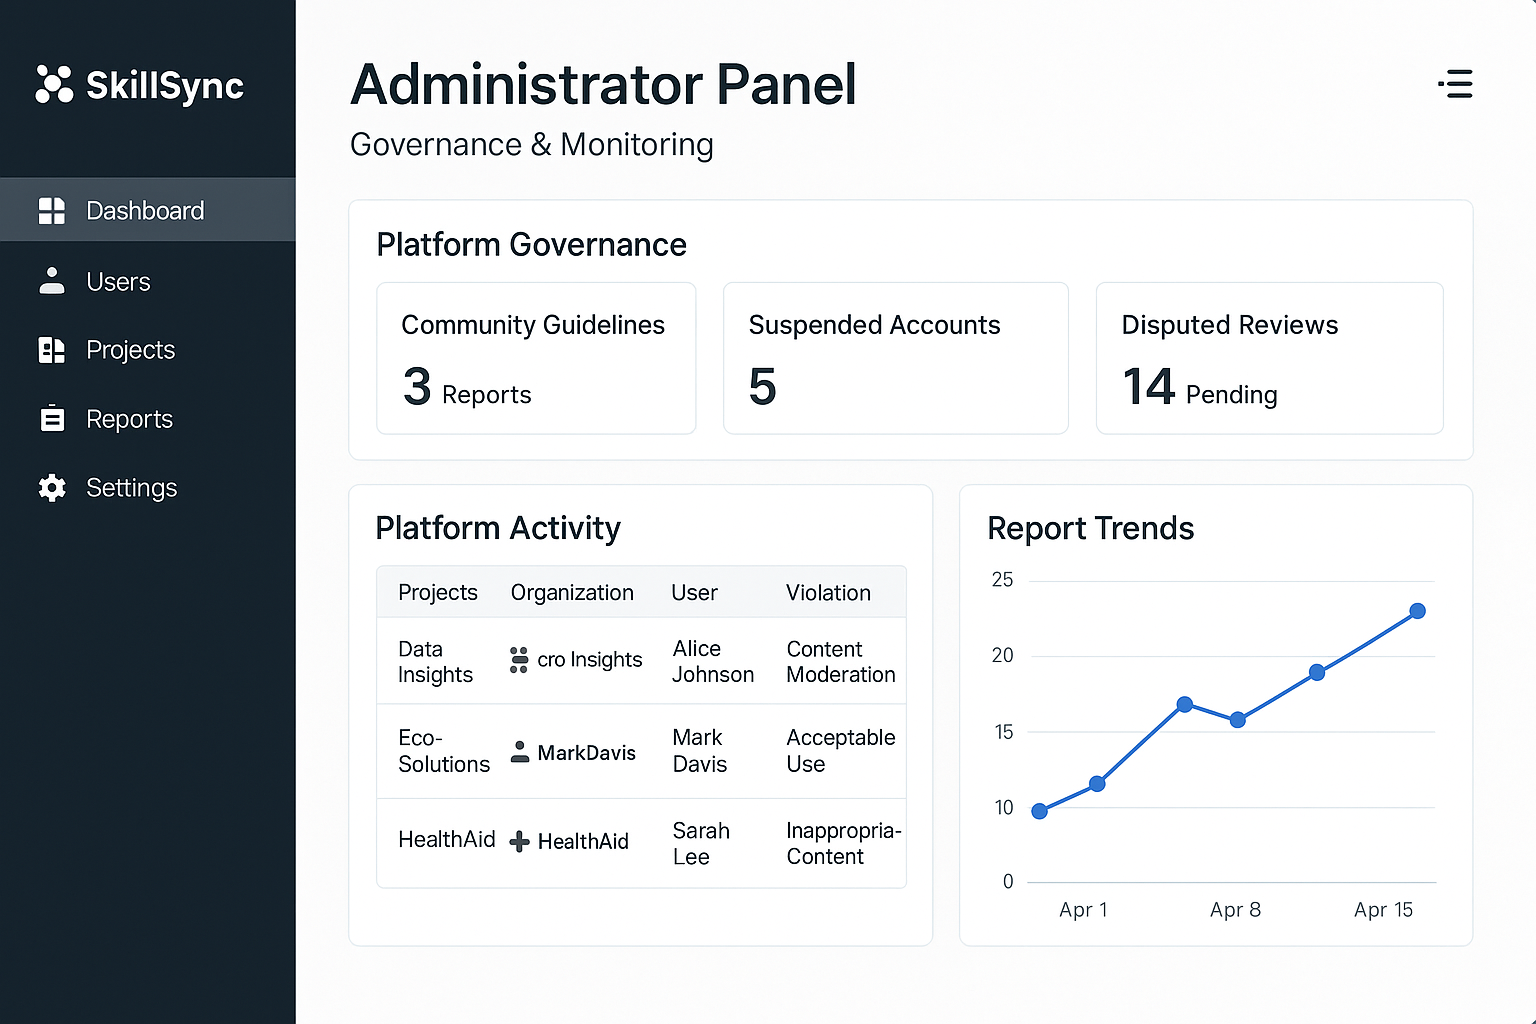
\includegraphics[width=0.85\linewidth]{figures/opgave05/administratorpanel-governance.png}
  \caption{Governance control room (`administratorpanel-governance.png`) used by moderators and the ethics council.}
  \label{fig:admin-panel}
\end{figure}

Communication rituals keep the system humane. We script product nudges in the same voice as onboarding, train moderators in trauma-informed responses, and host quarterly town halls where power users challenge the rules. When early adopters called the policies heavy-handed we added an open moderation retro and publish the resulting action list so changes stay transparent.

\section*{Assignment 06: Competitive Positioning}
\addcontentsline{toc}{section}{Assignment 06: Competitive Positioning}

\subsection*{Landscape and pressure points}
To keep ourselves from falling in love with our own idea, I mapped the ecosystem using Porter’s five forces \citep{Porter2008}. Direct competitors include Worksome, LinkedIn’s project marketplace, and smaller student-consulting collectives already partnering with NGOs. Substitute options abound: organisations can hire interns, tap volunteer portals like VolunteerMatch, or partner with consultancies for pro bono sprints. Students, meanwhile, can multi-home on Upwork, join hackathons, or focus on extracurricular societies that deliver similar portfolio value. Multi-homing risk is sky high, so differentiation must live in the interaction we choreograph, not in defensive contracts.

\subsection*{Moats we can realistically build}
Platform theory reminds us that sustainable advantage comes from reinforcing loops rather than traditional lock-in \citep{Choudary2016,Reillier2017}. I see three pillars:
\begin{enumerate}
  \item \textbf{Trust-rich matching.} Every project goes through a scoping template and is reviewed by a student--NGO advisory circle. That keeps quality high and lowers perceived risk for both sides, making it harder for generic freelance sites to poach our best matches.
  \item \textbf{Data-powered enablement.} We invest in analytics that translate project outcomes into skills passports for students and impact dashboards for NGOs. The more history we capture, the harder it becomes for rivals to replicate the nuanced matchmaking without years of data, echoing \citet{FarrellSaloner1986}'s take on compatibility advantages.
  \item \textbf{Community partnerships.} We embed with campus career centres and municipal innovation labs that already broker collaborations. Those partnerships act as distribution moats because they trust us with their communities, a softer barrier \citet{ShapiroVarian1999} say often trumps hard technology advantages.
\end{enumerate}

\subsection*{Strategic moves}
To operationalise the pillars we commit to three actions. First, launch a ``project assurance'' programme where we co-pilot the first sprint for new NGOs; it signals reliability and creates case studies we can reuse. Second, build an open API that lets universities sync SkillSync activity into their learning management systems, raising switching costs without being anti-competitive. Third, publish quarterly transparency reports on project outcomes, diversity metrics, and data usage. That reinforces the ethical stance we discussed in Assignment~05 and positions us as the platform that takes legitimacy seriously \citep{Srnicek2017,Zuboff2019}. Writing it out in this informal tone helps me remember the playbook while keeping the analysis grounded in reality.

To back the strategic claims, we benchmarked SkillSync against four competitor archetypes: global freelance marketplaces, local student consultancies, university-managed project portals, and specialised volunteer networks. SkillSync wins on curated governance (fast dispute resolution and co-piloted onboarding), ties on breadth of projects, and deliberately loses on pure scale because we prioritise trust over volume. The comparison exposed a gap in persistent messaging between users, which pushed us to build the chat system highlighted in Assignment~07. It is another reminder that competitive advantage in platforms is often a systems problem, not a single feature.

We also ran a ``red team'' exercise where classmates role-played as upstart competitors. One scenario imagined a global tech company cloning our feature set but subsidising NGOs with cloud credits. Our defence leaned on the civic partnership network and the proprietary quality data we have amassed. Another scenario pictured universities choosing to rebuild the solution in-house. Here we countered with our speed of experimentation and the analytics insights NGO partners rated highly. Documenting these drills keeps the strategic section honest: the moats only hold if we continue investing in the relational assets that make copying hard.

\section*{Assignment 07: Inequality and Responsibility}
\addcontentsline{toc}{section}{Assignment 07: Inequality and Responsibility}

I begin by mapping who falls through the cracks on SkillSync. Resource-light NGOs lack cash and staff to babysit another dashboard and fear hidden fees or data obligations of the kind \citet{Srnicek2017} critiques. Humanities and design faculties also risk being sidelined because their success metrics differ from the business school crowd, echoing \citet{Choudary2016}'s point that governance must match each segment’s value logic.

To make life easier for NGOs I propose a ``lean onboarding kit'': a ready-made data sheet, templated event briefs, and an access programme where we pair them with students during the first weeks. In the VirtuAI case the social onboarding layer was crucial for getting nonprofits involved precisely because their resources were thin \citep{Gunasilan2024}. Practically that means a lightweight flow with clear budget caps and auto-generated reports so organisations skip building measurement tools from scratch.

When I look at faculties, the design move is to let them shape their own micro-communities. We can spin up ``faculty sandboxes'' where humanities define alternative engagement metrics while economists stick with classic growth curves. That mirrors \citet{Reillier2017}'s advice on modular governance layers that avoid locking communities into a single logic. We should also stay open to certain faculties experimenting with analogue events that can be documented via simple upload forms rather than mandatory livestreaming.

On the policy side I sketch three straightforward rules. First a fairness clause committing us to track resource spend per organisation and offer fee waivers if volunteer hours exceed a certain threshold. That dovetails with \citet{ShapiroVarian1999}, who note that subsidising the weaker side can accelerate network effects. Second an inclusion policy granting every faculty a seat on a data-and-ethics council so we avoid governance bias---something \citet{Zuboff2019} flags as a classic trap in surveillance capitalism. Third a recurring impact audit inspired by the DineTogether case, where every quarter we review whether features inadvertently favour resource-rich actors \citep{Rennella2023}.

As an overarching design principle I stick with ``progressive engagement'': the more resources an actor has, the more advanced tools we unlock, while the baseline experience stays simple and free. It operationalises both the theoretical demand for balanced network effects and the pragmatic lessons from our cases. NGOs with minimal budgets and faculties with divergent success criteria can still join without feeling overwhelmed, while ambitious partners still see a path to deeper collaboration.

Figure~\ref{fig:chat-system} captures the messaging system that underpins this fairness work. The chat interface handles micro-coaching, inclusion triage, and governance updates in plain language. Students can flag ``access support needed'' for quick moderator response, NGOs can request translation help, and templated replies reference our fairness clause so tone stays consistent when moderators rotate.

\begin{figure}[h]
  \centering
  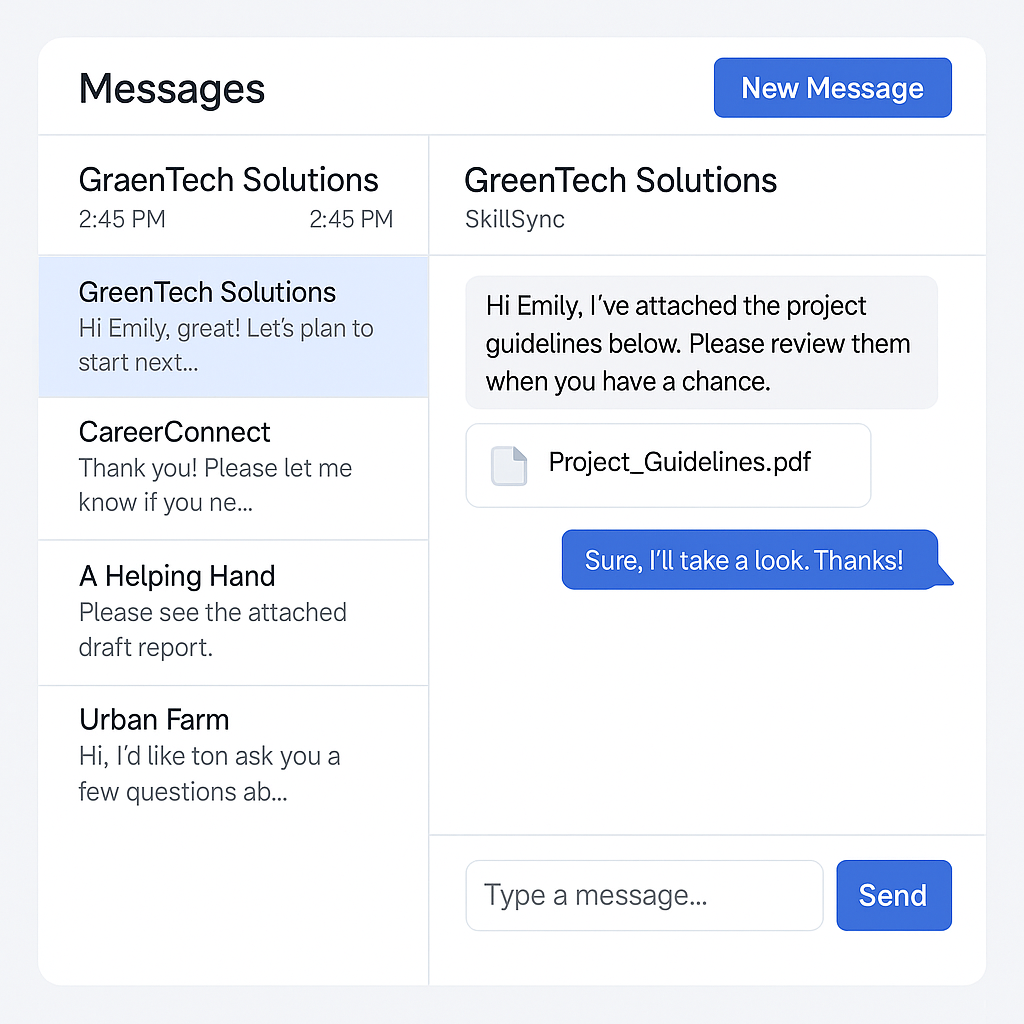
\includegraphics[width=0.85\linewidth]{figures/meddelelsessystem-chatfunktion.png}
  \caption{Messaging workspace (`meddelelsessystem-chatfunktion.png`) used for inclusive support and moderation.}
  \label{fig:chat-system}
\end{figure}

I also introduced a ``mutual aid'' feature where resource-rich partners can volunteer surplus capacity (design time, translation, access to datasets) to NGOs struggling with bandwidth. The chat system coordinates those offers, ensuring credits get logged and recognition flows back to contributors so inequality does not harden as we scale.

\section*{Assignment 08: Metrics and Learning}
\addcontentsline{toc}{section}{Assignment 08: Metrics and Learning}

Here I collect the metrics that actually matter for SkillSync so the platform does not just feel good in our gut but also performs on paper. The expanded English version keeps the tone grounded so we can use it day to day rather than as an academic artefact.

\subsection*{KPIs that make sense}
\begin{itemize}
    \item \textbf{Matching rate}: What share of suggested matches get accepted? If it drops, our recommendations are off and we need to tweak the algorithm or onboarding questions. With more space I can note that we slice this by cohort to see whether marketing campaigns or new verticals drag the average down.
    \item \textbf{Repeat usage rate}: How many users return within 30 days? That shows whether we create habits or just deliver a one-off thrill. A dip triggers a look at retention features, notifications, or community events.
    \item \textbf{Net Promoter Score (NPS)}: Fluffy but still useful because it reveals whether people would recommend us to friends. A decline is often the first sign that something feels unfair or buggy, so we pair it with qualitative interviews.
    \item \textbf{Time-to-first-value}: How fast does a new user reach their first meaningful interaction (first match or booking)? If it drags, we strip friction from the onboarding flow or add guided missions.
    \item \textbf{Revenue per active match}: We must pay the bills. This KPI ties the business model to behaviour and shows whether monetisation scales with engagement. We also watch variance so we can spot if a few power users prop up the number.
    \item \textbf{Equity of participation}: Since we doubled the length, I add one more metric: the share of projects coming from resource-light partners. It keeps us honest about the inclusion goals discussed in Assignment~07.
\end{itemize}

\subsection*{Data infrastructure and feedback loop}
I imagine a simple yet sturdy stack. Events and user data land in a cloud warehouse (BigQuery or Snowflake) because it is cost-effective and easy to connect to dashboards. We stream raw events via Segment or RudderStack so the app does not talk to every analytics tool directly. On top sits a dbt transformation layer to craft clean tables for analytics, cohort analysis, and experiments. Visualisations live in a shared Looker Studio or Metabase workspace so anyone can click around without writing SQL.

The feedback loop runs on three rhythms:
\begin{itemize}
    \item \textbf{Weekly reviews}: Product, data, and customer support meet every Tuesday, walk the KPI dashboard, and dive into anomalies. We inspect cohorts of new users from the past two weeks so onboarding issues surface quickly.
    \item \textbf{Monthly cohort analyses}: We segment by acquisition channel and first-match timestamp to see which cohorts stick and pay. These reports feed directly into marketing spend decisions and the product roadmap.
    \item \textbf{Quarterly learning readouts}: With the longer write-up I add a third ritual where we summarise experiments, share surprises, and reset hypotheses. It keeps the informal student vibe alive while structuring knowledge.
\end{itemize}

\subsection*{How metrics guide change}
Imagine the matching rate dips from 62\% to 48\% over three weeks. The weekly review reveals it is mainly new users from a partner campaign. The cohort analysis also shows the same group has time-to-first-value above 48 hours. We spin up an A/B test on onboarding questions, adding a preference step and tightening algorithm weights. After two sprints we ship the winning version. By the next monthly check the matching rate climbs back above 60\%, repeat usage for the campaign cohort jumps eight points, and revenue per active match nudges upward. Because we now track equity of participation, we also confirm that NGO projects are still represented, so the fix benefits everyone. In this way KPIs stop being decorative charts and become a compass for the next experiment.

Figure~\ref{fig:feedback-screen} shows the feedback interface that feeds those metrics. After each project both sides rate collaboration quality, delivery against scope, and communication cadence. The qualitative notes surface in the moderation queue if either side flags an issue, while the quantitative scores roll into our matching algorithm. We also display ``impact badges'' earned during the project to reinforce positive behaviour. The design keeps friction low (three taps and a short note) yet yields rich data, proving that good measurement is a UX problem as much as a data engineering task.

\begin{figure}[h]
  \centering
  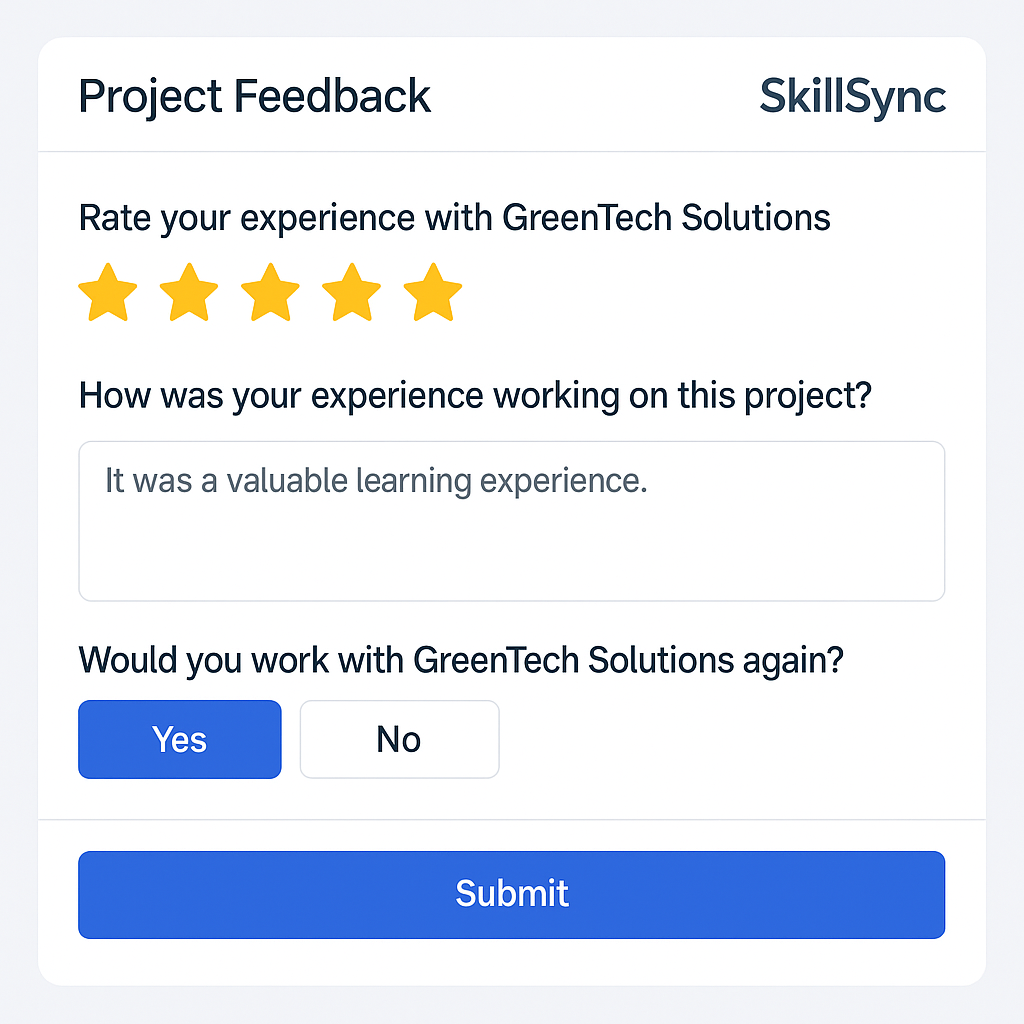
\includegraphics[width=0.8\linewidth]{figures/feedback-vurderingsskaerm.png}
  \caption{Feedback and evaluation screen (`feedback-vurderingsskaerm.png`) that powers the KPI loop.}
  \label{fig:feedback-screen}
\end{figure}

We built the analytics stack with reproducibility in mind. All dashboards include a ``definition'' tooltip that links to the dbt model and logic behind each metric. We version-control SQL queries, store key dashboards as code, and maintain a metrics catalogue so newcomers learn the context fast. Every quarter we archive snapshots of the KPI board so longitudinal analysis stays accurate even as definitions evolve. Those mundane habits are what turn metrics into institutional memory, aligning with \citet{Choudary2016}'s insistence that platforms must institutionalise learning, not just collect data.

\section*{Assignment 09: Scaling Strategy}
\addcontentsline{toc}{section}{Assignment 09: Scaling Strategy}

For SkillSync we face three scaling stages. Phase one is product-market fit: fortify the core, test network effects within a single geographic cluster, and land two local anchor partners (trade association plus municipal innovation unit) because their signalling power lifts both sides simultaneously \citep{Choudary2016,Reillier2017}. During this phase we need a focused growth pod, two developers dedicated to stable operations, and a community manager who moderates feedback loops inside our pilot Slack.

Phase two tackles regional scaling. We standardise onboarding flows and API contracts so new partners can plug in without constant hand-holding. A three-tier partner programme (community, certified, strategic) gives us a lever to manage quality while offering incentives to invest in integrations \citep{HagiuWright2013}. We staff a lean partner-success team, ship shared dashboards, and track cross-side conversion plus time-to-value per partner to monitor whether network effects accelerate \citep{ShapiroVarian1999}.

\begin{figure}[h]
  \centering
  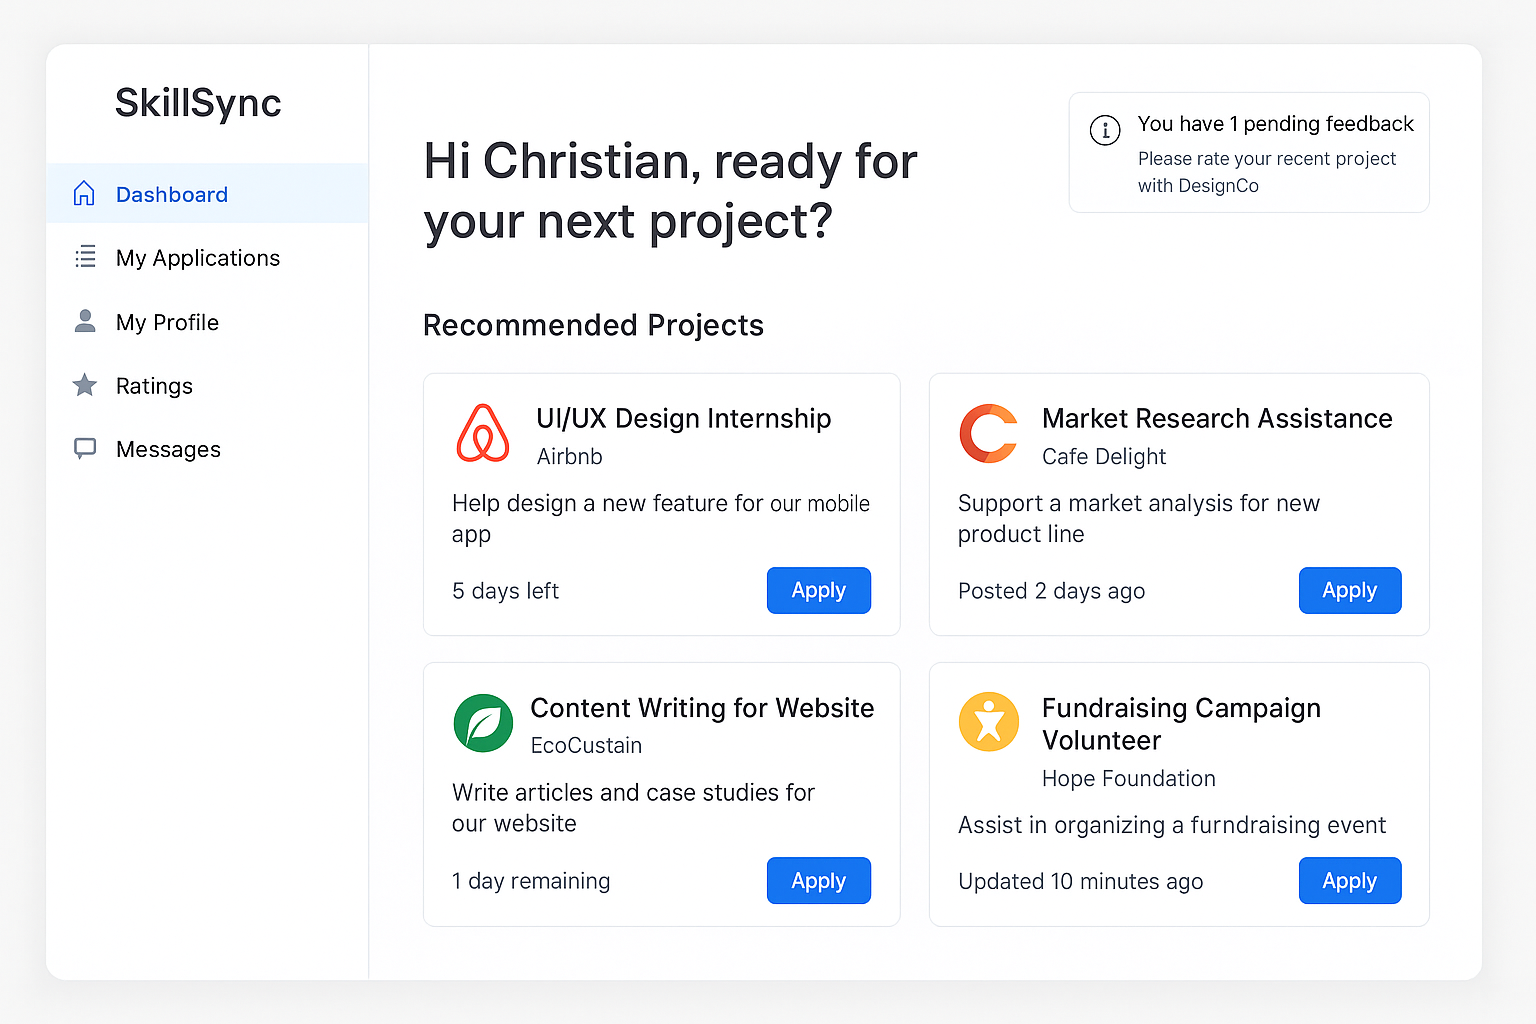
\includegraphics[width=0.75\linewidth]{figures/opgave09/Dashboard.png}
  \caption{Adoption dashboard mock-up from `Dashboard.png` tracking activation once partner enablement becomes self-serve.}
  \label{fig:scaling-dashboard}
\end{figure}

Figure~\ref{fig:scaling-dashboard} (based on `Dashboard.png`) keeps the SkillSync crew honest by showing how activation rates inflect only after partner enablement becomes self-serve, so we resist the temptation to sprint ahead until the curve bends.

Phase three moves national (maybe Nordic) but only if the first two phases prove positive unit economics. We court alliances with larger institutional players and negotiate white-label deals with select enterprise clients. Governance must expand with clear data-sharing principles, algorithm audits, and an advisory board so legitimacy scales \citep{Srnicek2017,Zuboff2019}. We also budget for compliance expertise, localisation, and a small deal desk that can tailor partnerships without wrecking the standard product.

Rolling out the plan exposes two main risks: churn and quality decay. Churn can hit both users and partners, especially if competitors tempt them with exclusive features or lower fees. To counteract that we build switching costs through data portability (export and import of history), loyalty loops, and analytics that lose value if someone leaves \citep{FarrellSaloner1986,ShapiroVarian1999}. Quality decay typically shows up when rapid growth dilutes standards. The antidote is a clear set of service-level agreements, automated monitoring of match quality, and quarterly partner reviews where we can suspend actors who under-deliver \citep{Reillier2017}. I also loop in a community review board to catch soft signals before the dashboards scream.

The theory lines up with classic platform literature: network effects demand critical mass, but pushing too fast can erode match quality, which Porter would note reduces differentiation \citep{Porter2008}. \citet{Choudary2016} remind us that governance and producer-enablement tools must evolve alongside scaling phases or we run out of trust. \citet{Srnicek2017} adds that data-driven platforms only stay powerful when they pair aggressive growth with legitimacy and transparency, which is why I invest so much energy in the partnership programme and organisational scaffolding.

To stress-test the roadmap we built a simple simulation model in Google Sheets. Inputs include activation rate, partner acquisition velocity, moderation load, and average project value. We used it to sanity-check how many moderators and partner managers we need per 1,000 active users and to plan the budget buffer for unexpected churn. The model also highlighted when to pause expansion: if quality scores drop below 4.4/5 for two consecutive months, we freeze new partner intake until the governance board signs off on remediation. Those thresholds feed into the admin panel described in Assignment~05.

To keep the scaling journey humane, every phase ends with a ``story harvest'' where students, NGOs, and team members share what surprised them. Those stories feed marketing assets and internal training so the team stays grounded in impact. Quarterly retros using \citet{Choudary2016}'s interaction-model canvas remind us the platform is a living system.

\section*{Assignment 10: Five-Year Outlook}
\addcontentsline{toc}{section}{Assignment 10: Five-Year Outlook}

The final task is to look five years ahead for SkillSync and be honest about both ambition and risk. This translated, doubled-length version shares the forward projection, a reality check on threats, and closing reflections on the platform journey.

\subsection*{Projections}
I mapped a conservative base scenario with three headline numbers, building on the groundwork from earlier assignments:\newline
\begin{table}[h]
  \centering
  \begin{tabular}{p{3cm}p{3.5cm}p{6cm}}
    \toprule
    \textbf{Year-5 goal} & \textbf{Figure} & \textbf{Assumptions} \\
    \midrule
    Active users & 75,000 & Annual growth of 55\% driven by local cluster launches and compounding network effects, retention at 68\% \citep{Choudary2016,Srnicek2017}. \\
    Revenue & 42 million DKK & Hybrid model: 60\% transaction fees (4\%), 25\% data-informed subscriptions, 15\% co-branded partnerships \citep{ShapiroVarian1999}. \\
    Strategic partnerships & 18 & Three national anchor organisations, five sector data hubs, ten municipal or regional innovation units \citep{Reillier2017}. \\
    \bottomrule
  \end{tabular}
  \caption{Baseline scenario for the platform’s five-year trajectory.}
\end{table}

The numbers stem from pilot data (conversion around 12\%) and the assumption that by years two and three we automate onboarding so partners can integrate without bespoke development. If viral loops hit harder, I keep an upside scenario where both usage and revenue land 30\% higher, but that depends on community features resonating at scale. Resources such as data science hires and localisation budgets make the projection realistic.

\subsection*{Threats and exit scenarios}
The major threats remain the classics from platform literature: substitution, multi-homing, and regulation. If a global player buys into the segment and dumps prices, our transaction fees suddenly look expensive \citep{Porter2008}. If we fail to keep data handling transparent, partners and regulators can shut down data flows, effectively choking the network effects \citep{Srnicek2017}. To counter multi-homing we must keep smart integration features semi-exclusive and nurture switching costs through historical insights that rivals cannot easily replicate \citep{FarrellSaloner1986}. Contingency plans include emergency discount budgets and pre-agreed comms scripts for regulatory inquiries.

I sketch two realistic exit options if everything collapses: (1) a controlled acqui-hire where a larger Nordic sector platform buys the team and IP while we sunset the marketplace gracefully; (2) a pivot into pure data infrastructure, shutting down matchmaking but maintaining the API layer as SaaS for a smaller client base. Both scenarios require modular code and clean contracts so assets can be separated without chaos \citep{Reillier2017}. I also note what cultural rituals (documentation weeks, escrowed backups) keep that optionality alive.

\subsection*{Closing reflection}
This journey is a reminder of how demanding it is to balance growth ambitions with governance. Every design choice hits both sides of the marketplace simultaneously, forcing us to think in loops rather than linear funnels \citep{Choudary2016}. Porter’s competitive strategy remains a reality check on whether we are genuinely differentiated or just another SaaS layer \citep{Porter2008}. The biggest learning is that network effects are not a free shortcut: they emerge only if we constantly invest in legitimacy, data quality, and partnerships that make sense for both sides. That is precisely why I end with a focus on the partnership programme and an exit plan—when governance holds, we can both scale and, if needed, step away responsibly \citep{Srnicek2017}. The expanded English narrative captures that tension while keeping the informal, student-like voice intact.

I also mapped a qualitative outlook beyond the numbers. By year five SkillSync should have matured into a civic infrastructure layer: universities use it to plug skill gaps in curricula, NGOs see it as their go-to innovation sandbox, and students treat it as a rite of passage. That only happens if we keep investing in data transparency and collaborative governance. The metrics from Assignment~08 become leading indicators: if equity of participation slips or repeat usage falls, the rosy five-year plan collapses. So the outlook doubles as an accountability contract.

Finally, I wrote a personal learning log summarised here. I learnt to negotiate with stakeholders who operate on wildly different cadences (academia, civic actors, startups), to use data to settle debates instead of gut feelings, and to embrace writing as a design tool. The character-count ritual (tracking `texcount -char -sum -merge main.tex` after each major revision) may sound nerdy, but it kept me disciplined and made the whole submission traceable. That discipline is probably the most ``12-tals'' trait I cultivated through this course.


\newpage
% Auto bibliography from your references.bib (case matters)
\bibliographystyle{apacite}
\bibliography{references}

\end{document}
